% This is the root file of your thesis: thesis.tex
% A line starting with % is a comment. In some cases, I have included a command preceded by a %. You may activate the command by removing the %.

%%===================================
%%%%%%%%%%%%%%%%%%%%%%%%%%%%%%%%%%%%%%%%%%%%%%%%%%%%%%%%%%%%%%%%%%
%                           Document style
%%%%%%%%%%%%%%%%%%%%%%%%%%%%%%%%%%%%%%%%%%%%%%%%%%%%%%%%%%%%%%%%%%

\documentclass[12pt]{report}
\usepackage{ramsstyle}
%%===================================
%Write the various parts of your thesis as separate files and include them into the main file by the command \include{name of included file}. When you compile the LaTeX file, you may choose which subfiles to include by the command

%\includeonly{chapter01,chapter02}

%%===================================
\begin{document}
%%%%%%%%%%%%%%%%%%%%%%%%%%%%%%%%%%%%%%%%%%%%%%%%%%%%%%%%%%%%%%%%%%
%                   Command for the first page 
%%%%%%%%%%%%%%%%%%%%%%%%%%%%%%%%%%%%%%%%%%%%%%%%%%%%%%%%%%%%%%%%%%

\newcommand*\FirstPage{
\thispagestyle{empty}
% placing a pdf as background and adding text on top

\includepdf[pages=1,picturecommand*={ 
                % selecting placement, font size and text type
                \put(130,630){\fontsize{28}{28}\selectfont{\textsc{\textbf{Spicy Title}}}}
                \put(130,200){\fontsize{28}{28}\selectfont{\Large{\textbf{Teknisk rapportmal}}}}
                \put(130,180){\fontsize{28}{28}\selectfont{\Large{\textbf{NTNU studenter}}}}
                \put(130,160){\fontsize{28}{28}\selectfont{\Large{\textbf{Trondheim, vår 2020}}}}
                }]{images/ntnu_front_page.pdf}}

%This is the Titlepage
%%=========================================
\thispagestyle{empty}
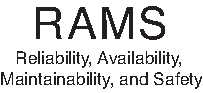
\includegraphics[scale=1.1]{fig/rams}
\mbox{}\\[6pc]
\begin{center}
\Huge{Resilience to Sea Level Extremes in Trondheim}\\[2pc]

\Large{Amy Anne McCormack}\\[1pc]
\large{Novermber 2022}\\[2pc]

PROJECT THESIS\\
Department of Geography\\
Norwegian University of Science and Technology
\end{center}
\vfill

\noindent Supervisor 1: Associate Professor Chantel Nixon

\noindent Supervisor 2: Associate Professor Martina Calovi

 % This is the titlepage
\setcounter{page}{0}
\pagenumbering{roman}
%document preamble 
\documentclass{article}
\usepackage{graphicx}
\usepackage{array}
\graphicspath{ {figures/} }
\begin{document}
%This is the Preface
%%=========================================

%attempting to insert signature as picture
\addcontentsline{toc}{section}{Preface}{Unnumbered Section}
\section{Preface}


%\addcontentsline{toc}{section}{Preface}
\title{Preface}
This is a Master's thesis completed as part of the study program Natural Resources Management MSc at NTNU in the deparment of Geography. It was carried out in 2022 with data collection occurring during the summer. The idea for the project occurred to the researcher during a kayaking expedition in Lofoten where she came across many individuals with direct memory and experience of sea level change and extreme sea levels. \\[2cm]

\begin{center}
Trondheim, 2022-11-15\\[1pc]


Amy Anne McCormack 
\end{center}



\graphicspath{ {./images/} }

\includegraphics[scale=0.5]{fig/to use signature png}
\newpage

%% insert table of contents
\tableofcontents

%rename figure list and table list 
\renewcommand{\listfigurename}{List of Figures}
\renewcommand{\listtablename}{List of Tables}

%insert figure list
%insert table list
\listoffigures
\listoftables
\clearpage
\pagenumbering{arabic}



word words words


\end{document}

%This is the Acknowledgment
%%=========================================
\addcontentsline{toc}{section}{Acknowledgment}
\section*{Acknowledgment}
I would like to thank the following persons for their great help during this project. Chantel Nixon, Martina Cavoli. Callum Sinclair. NARM writing group. Everyone who brought me a cup of tea as I wrote this. \ldots



\begin{flushright}
A.A.M\\[1pc]

\end{flushright}
%This is the Summary
%%=========================================
\addcontentsline{toc}{section}{Summary and Conclusions}
\section*{Summary and Conclusions}
Here you give a summary of your your work and your results. This is like a management summary and should be written in a clear and easy language, without many difficult terms and without abbreviations. Everything you present here must be treated in more detail in the main report. You should not give any references to the report in the summary -- just explain what you have done and what you have found out. The Summary and Conclusions should be no more than two pages.
\tableofcontents
\setcounter{page}{0}
\pagenumbering{arabic}
%This is chapter 1
%%=========================================
\chapter{Introduction}
The first chapter of a well-structured thesis is always an introduction, setting the scene with background, problem description, objectives, limitations, and then looking ahead to summarize what is in the rest of the report. This is the part that readers look at first---\emph{so make sure it hooks them!}

%%=========================================
\section{Background}
In this section, you should present the problem that you are going to investigate or analyze; why this problem is of interest; what has, so far, been done to solve the problem, and which parts of the problem that remain.
%%=========================================
\subsection*{Problem Formulation}
You should define your problem in a clear an unambiguous way and explain why this is a problem, why it is of interest---and to whom. It is also important to delimit the problem area.
%%=========================================
\subsection*{Literature Survey}
You should here present the main books and articles that treat problems that are similar to what  you are studying. If you,  later in your thesis, describe the ``state of the art'' -- with a detailed literature survey, you may just give a very brief survey here (approx. a quarter of a page). If this is the only literature survey, you need to go into more details. An objective of the literature survey is to show the reader that you are familiar with the main literature within your field of research -- so that you do not ``reinvent the wheel.''


References to literature can be given in two different ways:
\begin{itemize}
\item As an \emph{explicit} reference: It is shown by \citet{lundteigen08} and partly also by \citet{rausand04}  that \ldots.
\item As an \emph{implicit} reference: It is shown \citep[e.g., see][Chap. 4]{rausand04} that \ldots.
\end{itemize}
In the example above, we have used ``author-year'' references, which is the preferred format. 
\begin{remark}
Following agreement with your supervisor, you may also refer by numbers, for example,  [1]. To do this, open the file \texttt{ramsstyle.sty} and  comment out (by \%) the command \texttt{$\backslash$usepackage\{natbib\}} and un-comment the corresponding command \texttt{$\backslash$usepackage[numbers]\{natbib\}}.\footnote{Notice the strange way we have to write the ``backslash'' in the text. This is because the ``backslash'' is a command in \LaTeX.}
\end{remark}
 You may include a link to the Internet in the text or in a footnote by using a command like: \url{http://www.ntnu.edu/ross}. 

When you refer to the scientific literature, you should always write in \emph{present} tense. Example: \citet{rausand04} show that \ldots.

\begin{remark}
Hyperlinks are included by the command \texttt{$\backslash$usepackage\{hyperref}\} in \texttt{ramsstyle.sty}. If you feel that the hyperlinks are disturbing when you enter the text, or want to avoid the hyperlinks in printed text, you may either comment out or edit this command in \texttt{ramsstyle.sty}.
\end{remark}
%%=========================================
\subsection*{What Remains to be Done?}
After you have defined and delimited your problem -- and presented the relevant results found in the literature within this field, you should sum up which parts of the problem that remain to be solved.
%%=========================================
\section{Objectives}
The main objectives of this Master's project are
\begin{enumerate}
\item This is the first objective
\item This is the second objective
\item This is the third objective
\item More objectives
\end{enumerate}

All objectives shall be stated such that we, after having read the thesis, can see whether or not you have met the objective. ``To become familiar with \ldots'' is therefore not a suitable objective.

%%=========================================
\section{Limitations}
In this section you describe the limitations of your study. These may be related to the study object (physical limitations, operational limitations), to the thoroughness of the analysis, and so on.
%%=========================================
\section{Approach}
Here you should describe the (scientific) approach that you will use to solve the problem and meet your objectives. You should specify the approach for each objective.

If there are any ethical problems related to your approach, these should be highlighted and discussed.
%%=========================================
\section{Structure of the Report}
The rest of the report is structured as follows. Chapter 2 gives an introduction to \ldots

\begin{remark}
Notice that chapter and section headings shall be written in lowercase, but that all main words should start with a capital letter.
\end{remark}


The report should be no longer than \underline{60 pages} in this format (+ the CV).
%This is chapter 2
%%=========================================
\chapter[Equations, etc]{Equations, Figures, and Tables}
The content of this chapter will vary with the topic of your thesis. 
\begin{remark}
If you want a shorter chapter or section title to appear in the Table of Contents and in the headings of the chapter, you just include the short title in square brackets before the title of the chapter/section.
\end{remark}

%%=========================================
\section{Simple Equations}
This is how a simple equation is included:
\begin{equation}
F(t)=\int_0^t \exp(-\lambda x)\,dx
\label{eq1}
\end{equation}

The equations are automatically given equation numbers -- here (\ref{eq1}) since this is the first equation in Chapter 2. Note that you can refer to the equation by referring to the ``label'' you specified as part of the equation environment.

You can also include equations without numbers:
\begin{equation*}
F(t)=\sum_{i=1}^n \binom{n}{i}\sin(i\cdot t)
\end{equation*}

%%=========================================
\subsection*{More Advanced Formulas}
Please consult the \LaTeX\ documentation.

If you want to include a definition of a term/concept in the text, I have made the following macro (see in \texttt{ramsstyle.sty}):
\begin{defin}
\textbf{Reliability}: The ability of an item to perform a required function under stated environmental and operational conditions and for a stated period of time.
\end{defin}

%%=========================================
\section{Including Figures}
If you use pdf\LaTeX\ (as recommended), all the figures must be in pdf, png, or jpg format. We recommend you to use the pdf format.  Please place the figure files in the directory \textbf{fig}. Figures are included by the command shown for Figure~\ref{fig1}. Please notice the ``path'' to the figure file written by a \emph{forward} slash (/). You should not include the format of the figure file (pdg, png, or jpg) -- just write the ``name'' of the figure. 
\begin{figure}
\centering

\includegraphics[scale=0.6,angle=15]{fig/NTNU}
\caption{This is the logo of NTNU (rotated 15 degrees).}
\label{fig1}
\end{figure}

Each figure should include a unique \emph{label} as shown in the command for Figure~\ref{fig1}. You can then refer to the figure by the \emph{ref} command.
Notice that you can scale the size of the figure by the option \texttt{scale=k}. You may also define a specific width or height of the figure by replacing the \texttt{scale} options by \texttt{width=k} or \texttt{height=k}. The factor \texttt{k} can here be specified in mm, cm, pc, and many other length measures. You may also give \texttt{k} as a fraction of the width of the text or of the height of the text, for example, \texttt{width=0.45$\backslash$textwidth}. If you later change the margins of the text, the figure width will change accordingly. As illustrated in Figure~\ref{fig1}, you may also rotate the figure -- and also do many other things (please check the documentation of the package \texttt{graphicx} -- it is available on your computer, or you may find it on the Internet).

In \LaTeX\ all figures are floating objects and will normally be placed at the top of a page. This is the standard option in all scientific reports. If you insist on placing the figure exactly where you declare the figure, you may include the command \texttt{[h]} (here) immediately after $\backslash$\texttt{begin\{figure\}}. If you will force the figure to be located either at the top or bottom of the page, you may alternatively use  \texttt{[t]} or \texttt{[b]}. For more options, check the documentation.

Large figures may be included as a \emph{sidewaysfigure} as shown in Figure~\ref{fig2}:\footnote{You can use a similar command for large tables.}
\begin{sidewaysfigure}
\centering

\includegraphics[scale=1.8]{fig/NTNU}
\caption{This is the logo of NTNU.}
\label{fig2}
\end{sidewaysfigure}

%%=========================================
\section{Including Tables}
\LaTeX\ has a lot of different options to include tables. Only one of them is illustrated here.

\begin{table}
	\centering\small
	\caption{The degree of newness of technology.}
	\label{tab1}
		\begin{tabular*}{\textwidth}{@{\extracolsep{\fill}}lccc}
			\toprule
			  &\multicolumn{3}{c}{Level of technology maturity}\\
  \cmidrule{2-4}
			Experience with the		   &  & Limited field history or not & New or \\
              operating  condition  & Proven &  used by company/user & unproven \\
        
			\midrule
			  Previous experience & 1 & 2 & 3 \\
		          No experience by company/user & 2 & 3 & 4 \\
		          No industry experience & 3 & 4 & 4 \\
			\bottomrule
		\end{tabular*}
\end{table}

\begin{remark}
Notice that figure captions (Figure text) shall be located \emph{below} the figure -- and that the caption of tables shall be \emph{above} the table. This is done by placing the $\backslash$\texttt{caption} command beneath the command $\backslash$\texttt{includegraphics} for figures, and above the command $\backslash$\texttt{begin\{tabular*\}} for tables.
\end{remark}
%%=========================================
\section{Copying Figures and Tables}
In some cases, it may be relevant to include figures and tables from from other publications in your report. This can be a direct copy or that you retype the table or redraw the figure. In both cases, you should include a reference to the source in the figure or table caption. The caption might then be written as: \textsl{Figure/Table xx: The caption text is coming here \citep{rausand04}.}

In other cases, you get the idea from a figure or table in a publication, but modify the figure/table to fit your purpose. If the change is significant, your caption should have the following format: \textsl{Figure/Table xx: The caption text is coming here \citep[adapted from][]{rausand04}.}

%%=========================================
\section{References to Figures and Tables}
Remember that all figures and tables shall be referred to and explained/discussed in the text. If a figure/table is not referred to in the text, it shall be deleted from the report.
%%=========================================
\section{A Word About Font-encoding}
When you press a button (or a combination of buttons) on your keyboard, this is represented in your computer according to the \emph{font-encoding} that has been set up. A wide range of font-encodings are available and it may be difficult to choose the ``best'' one. In the template, I have set up a font-encoding called UTF-8 which is a modern and very comprehensive encoding and is expected to be the standard encoding in the future. Before you start using this template, you should open the Preferences ->Editor dialogue in TeXworks (or TeXShop if you use a Mac) and check that encoding UTF-8 has been specified. 

If you use only numbers and letters used in standard English text, it is not very important which encoding you are using, but if you write the Norwegian letters æ, ø, å and accented letters, such as é and ä, you may run into problems if you use different encodings. Please be careful if you cut and paste text from other word-processors or editors into your \LaTeX\ file!

\subsubsection*{Warning}
If you (accidentally) open your file in another editor and this editor is set up with another font-encoding, your non-standard letters will likely come out wrong. If you do this, and detect the error, be sure \emph{not} to save your file in this editor!!

This is not a specific \LaTeX\ problem. You will run into the same problem with all editors and word-processors -- and it is of special importance if you use computers with different platforms (Windows, OSX, Linux).

%%=========================================
\section{Plagiarism}
Plagiarism is defined as ``use, without giving reasonable and appropriate credit to or acknowledging the author or source, of another person's original work, whether such work is made up of code, formulas, ideas, language, research, strategies, writing or other form'', and is a very serious issue in all academic work. You should adhere to the following rules:
\begin{itemize}
\item Give proper references to all the sources you are using as a basis for your work. The references should be give to the original work and not to newer sources that mention the original sources.
\item You may copy paragraphs up to 50 words when you include a proper reference. In doing so, you should place the copied text in inverted commas (i.e., ``Copied text follows \ldots''). Another option is to write the copied text as a quotation, for example:
\begin{quote}
Birnbaum's measure of reliability importance of component $i$ at time $t$ is equal to the probability that the system is in such a state at time $t$ that component $i$ is critical for the system.\newline \mbox{} \hfill \citet{rausand04}
\end{quote}
\end{itemize}




%This is the last chapter 
%%=========================================
\chapter[Summary]{Summary and Recommendations for Further Work}

In this final chapter you should sum up what you have done and which results you have got. You should also discuss your findings, and give recommendations for further work.

%%=========================================
\section{Summary and Conclusions}
Here, you present a brief summary of your work and list the main results you have got. You should give comments to each of the objectives in Chapter 1 and state whether or not you have met the objective. If you have not met the objective, you should explain why (e.g., data not available, too difficult).

This section is similar to the Summary and Conclusions in the beginning of your report, but more detailed---referring to the the various sections in the report.

%%=========================================
\section{Discussion}
Here, you may discuss your findings, their strengths and limitations.
%%=========================================
\section{Recommendations for Further Work}
You should give recommendations to possible extensions to your work. The recommendations should be as specific as possible, preferably with an objective and an indication of a possible approach.

The recommendations may be classified as:
\begin{itemize}
\item Short-term
\item Medium-term
\item Long-term
\end{itemize}
% Include more chapters as required.
%%=========================================
\appendix
%This is Appendix A - Acronyms
%%=========================================

\chapter{Acronyms}
\begin{description}
\item[df]degrees of freedom
\item[GIA] glacioisostatic adjustment
\item[No.] Number of
\item [RStudio] RStudio Version 2022.02.3+492 on Windows Desktop
\item[SLEs] Sea Level Extremes
\item [UN SDGs] United Nations Sustainable Development Goals 
\end{description}

Note that if there is a variation in English spelling the British English variation was selected in line with the Cambridge Dictionary. For SI units the UK metric organisation style guide was followed https://ukma.org.uk/style-guide/.  

The code used can be found in the github repo: 
%This is an Appendix
%%=========================================

\chapter{Hypotheses, Summary Statistics, Visual Communication}

%%=========================================
\section{Hypotheses}

\subsection{Hypothesis dependent on community membership}
\begin{enumerate}
    \item We expect residents to be aware
    \item We expect commuters to be aware
    \item We expect marine workers to be aware
    \item We expect non-marine workers to be unaware
    \item We expect water leisure users to be aware
    \item We expect land leisure users to be unaware
    \end{enumerate}
\paragraph{}

\subsection{Hypothesis dependent on local knowledge}
\begin{enumerate}
    \item We expect subjects with professional interest in SLEs to be aware
    \item We expect subjects with primary knowledge about places which are on reclaimed land to be aware
    \item We expect subjects with a length of knowledge greater than 20 years of the area to be aware
    \item We expect subjects with a length of knowledge less than 1 year of the area to be unaware
    \item We expect subjects with many information sources about the place to be aware
    \item We expect subjects who chose to respond in Norwegian to be aware
\end{enumerate}
\paragraph{}

\subsection{Hypothesis dependent on awareness of changing climate}
\begin{enumerate}
    \item We expect subjects with many information sources about climate change to be aware
    \item We expect subjects with the information source of formal education to be aware
    \item We expect subjects with the information source of peer reviewed published papers to be aware
    \item We expect subjects who are more concerned about climate change to be aware
    \item We expect subjects who predict they will be impacted by flooding from SLEs to be aware
\end{enumerate}

\section{Summary Statistics }
Find below table \ref{table:summary_stats} which details the summary statistics for the responses to the survey. Table \ref{table:variable to questions} contains the codified variable name and what questions they respond to.



\begin{center}
\begin{table}[H]
    \centering
    \begin{tabular}{|l|l|l|l|l|l|l|}
    \hline
        variable name & mean & Std Dev. & min & max & range & skew  \\ \hline
        long\_know & 3.24 & 1.60 & 0 & 6 & 6 & 0.23 \\ \hline
        com\_mem & 1.44 & 0.89 & 0 & 6 & 6 & 2.10  \\ \hline
        com\_marine\_worker & 0.00 & 0.00 & 0 & 0 & 0 & Na   \\ \hline
        com\_worker & 0.12 & 0.33 & 0 & 1 & 1 & 2.26  \\ \hline
        com\_resident & 0.46 & 0.50 & 0 & 1 & 1 & 0.17  \\ \hline
        com\_student & 0.25 & 0.44 & 0 & 1 & 1 & 1.11 \\ \hline
        com\_play\_land & 0.27 & 0.45 & 0 & 1 & 1 & 1.00   \\ \hline
        com\_play\_water & 0.11 & 0.32 & 0 & 1 & 1 & 2.45  \\ \hline
        com\_commuter & 0.10 & 0.31 & 0 & 1 & 1 & 2.56   \\ \hline
        com\_other & 0.12 & 0.32 & 0 & 1 & 1 & 2.35   \\ \hline
        interest\_level & 3.17 & 0.95 & 1 & 5 & 4 & -0.16 \\ \hline
        ss\_now & 0.39 & 0.49 & 0 & 1 & 1 & 0.44  \\ \hline
        ss\_future & 0.31 & 0.46 & 0 & 1 & 1 & 0.83 \\ \hline
        ss\_tide & 0.88 & 0.32 & 0 & 1 & 1 & -2.35 \\ \hline
        info\_place\_sum & 1.94 & 1.34 & 0 & 8 & 8 & 1.61 \\ \hline
        info\_climate\_sum & 3.50 & 1.72 & 0 & 8 & 8 & 0.24 \\ \hline
        worry\_climate & 4.03 & 1.15 & 1 & 5 & 4 & -1.17 \\ \hline
        flood\_impact & 2.50 & 0.89 & 1 & 4 & 3 & 0.04  \\ \hline
        slr\_past & 0.17 & 0.43 & 0 & 2 & 2 & 2.47  \\ \hline
        slr\_future & 2.33 & 0.69 & 0 & 3 & 3 & -1.26 \\ \hline
        ss\_event & 0.58 & 0.93 & 0 & 7 & 7 & 2.78  \\ \hline
        survey\_access & 2.55 & 1.84 & 0 & 6 & 6 & 0.79  \\ \hline
        language & 0.57 & 0.50 & 0 & 1 & 1 & -0.27  \\ \hline
        place\_brattøra & 0.20 & 0.40 & 0 & 1 & 1 & 1.52  \\ \hline
        place\_grillstad & 0.24 & 0.43 & 0 & 1 & 1 & 1.19 \\ \hline
        place\_nidelva & 0.37 & 0.49 & 0 & 1 & 1 & 0.52 \\ \hline
        place\_skansen & 0.19 & 0.39 & 0 & 1 & 1 & 1.57 \\ \hline
    \end{tabular}
    \caption{Summary Statistics}
\label{table:summary_stats}
\end{table}
\end{center}


\begin{center}
\begin{table}[H]
    \centering
    \begin{tabular}{|l|l|}
    \hline
        variable name  & question asked \\ \hline
        long\_know & How long have you known this area? \\ \hline
        com\_mem  & What communities in this area are you part of? \\ \hline
        com\_marine\_worker & "" \\ \hline
        com\_worker & "" \\ \hline
        com\_resident & "" \\ \hline
        com\_student & "" \\ \hline
        com\_play\_land & "" \\ \hline
        com\_play\_water &  "" \\ \hline
        com\_commuter &  "" \\ \hline
        com\_other &  "" \\ \hline
        interest\_level & What is your level of interest in sea level extremes? \\ \hline
        ss\_now  & Which image shows the current 20-year storm surge? \\ \hline
        ss\_future  & Which image shows the 20-year storm surge projected for 2090? \\ \hline
        ss\_tide  & Which image displays the current high tide? \\ \hline
        info\_place\_sum & Where do you get information about changes to this place? \\ \hline
        info\_climate\_sum &  "Where do you get information about changes to the climate" \\ \hline
        worry\_climate &  Are you concerned about climate change? \\ \hline
        flood\_impact &  How would flooding associated with sea level extremes in this area affect you? \\ \hline
        slr\_past & How much do you think the sea level has changed here in the past 30 years? \\ \hline
        slr\_future & How much do you think the sea level will change in the next 30 years? \\ \hline
        ss\_event & Please tick if you remember any of these dates when coastal  \\ \newline
        & sea levels in Trondheim were over 2m \\ \hline
        survey\_access  & How did you access this survey? \\ \hline
        language  & Determined from which survey subjects filled out \\ \hline
        place\_brattøra  & "" \\ \hline
        place\_grillstad  & "" \\ \hline
        place\_nidelva & "" \\ \hline
        place\_skansen & "" \\ \hline
    \end{tabular}
    \caption{Variable link to Survey Question}
\label{table:variable to questions}
\end{table}
\end{center}


\begin{center}
\begin{table}[H]
    \centering
    \begin{tabular}{|l|l|l|l|l|l|l|}
    \hline
        variable name & mean & Std Dev. & min & max & range & skew  \\ \hline
        info\_place\_sum & 1.94 & 1.34 & 0 & 8 & 8 & 1.61 \\ \hline
        info\_place\_po & 0.73 & 0.45 & 0 & 1 & 1 & -1.00  \\ \hline
        info\_place\_family & 0.10 & 0.31 & 0 & 1 & 1 & 2.56 \\ \hline
        info\_place\_friend & 0.19 & 0.39 & 0 & 1 & 1 & 1.57  \\ \hline
        info\_place\_newspaper & 0.35 & 0.48 & 0 & 1 & 1 & 0.64  \\ \hline
        info\_place\_tv & 0.14 & 0.35 & 0 & 1 & 1 & 2.09 \\ \hline
        info\_place\_so\_me & 0.33 & 0.47 & 0 & 1 & 1 & 0.73  \\ \hline
        info\_place\_mem & 0.04 & 0.19 & 0 & 1 & 1 & 4.70 \\ \hline
        info\_place\_kommune & 0.07 & 0.26 & 0 & 1 & 1 & 3.28\\ \hline
        info\_climate\_sum & 3.50 & 1.72 & 0 & 8 & 8 & 0.24  \\ \hline
        info\_climate\_po & 0.45 & 0.50 & 0 & 1 & 1 & 0.20 \\ \hline
        info\_climate\_family & 0.18 & 0.38 & 0 & 1 & 1 & 1.68  \\ \hline
        info\_climate\_friend & 0.23 & 0.42 & 0 & 1 & 1 & 1.28  \\ \hline
        info\_climate\_newspaper & 0.72 & 0.45 & 0 & 1 & 1 & -0.96 \\ \hline
        info\_climate\_tv & 0.46 & 0.50 & 0 & 1 & 1 & 0.14 \\ \hline
        info\_climate\_so\_me & 0.63 & 0.48 & 0 & 1 & 1 & -0.55 \\ \hline
        info\_climate\_mem & 0.14 & 0.35 & 0 & 1 & 1 & 2.09 \\ \hline
        info\_climate\_sci & 0.39 & 0.49 & 0 & 1 & 1 & 0.44 \\ \hline
        info\_climate\_edu & 0.29 & 0.46 & 0 & 1 & 1 & 0.89 \\ \hline
        
         \end{tabular}
    \caption{Summary Statistics information access}
\label{table:summary_stats_info_access}
\end{table}
\end{center}

questions asked Where do you get information about this place? Where do you get information about climate change?
\begin{center}
\begin{table}[H]
    \centering
    \begin{tabular}{|l|l|l|l|l|l|l|}
    \hline
        variable name & mean & Std Dev. & min & max & range & skew \\ \hline
        risk\_p\_none & 0.46 & 2.10 & 0 & 10 & 10 & 4.31\\ \hline
        risk\_p\_he & 0.41 & 0.81 & 0 & 2 & 2 & 1.47 \\ \hline
        risk\_p\_drown & 0.72 & 0.96 & 0 & 2 & 2 & 0.58  \\ \hline
        risk\_p\_coldw & 0.24 & 0.65 & 0 & 2 & 2 & 2.35  \\ \hline
        risk\_p\_shore\_slide & 0.43 & 0.50 & 0 & 1 & 1 & 0.27 \\ \hline
        risk\_p\_ss & 0.57 & 0.50 & 0 & 1 & 1 & -0.27  \\ \hline
        risk\_p\_waves & 0.29 & 0.46 & 0 & 1 & 1 & 0.89 \\ \hline
        risk\_p\_wind & 0.34 & 0.48 & 0 & 1 & 1 & 0.67  \\ \hline
        risk\_p\_tide & 0.39 & 0.49 & 0 & 1 & 1 & 0.47  \\ \hline
        risk\_p\_storm\_total & 2.02 & 1.47 & 0 & 5 & 5 & 0.26  \\ \hline
        risk\_i\_dk & 0.72 & 2.59 & 0 & 10 & 10 & 3.28  \\ \hline
        risk\_i\_none & 0.26 & 1.60 & 0 & 10 & 10 & 5.88 \\ \hline
        risk\_i\_weathering & 1.08 & 1.44 & 0 & 3 & 3 & 0.58  \\ \hline
        risk\_i\_rain & 0.75 & 1.30 & 0 & 3 & 3 & 1.15\\ \hline
        risk\_i\_he & 0.35 & 0.76 & 0 & 2 & 2 & 1.68 \\ \hline
        risk\_i\_shore & 0.50 & 0.50 & 0 & 1 & 1 & -0.01 \\ \hline
        risk\_i\_ss & 0.63 & 0.48 & 0 & 1 & 1 & -0.55  \\ \hline
        risk\_i\_wave & 0.33 & 0.47 & 0 & 1 & 1 & 0.70  \\ \hline
        risk\_i\_wind & 0.31 & 0.46 & 0 & 1 & 1 & 0.83 \\ \hline
        risk\_i\_tide & 0.37 & 0.48 & 0 & 1 & 1 & 0.55  \\ \hline
        risk\_i\_storm\_total & 2.14 & 1.51 & 0 & 5 & 5 & 0.33 \\ \hline
          \end{tabular}
    \caption{Summary Statistics Perceived Risks}
\label{table:summary_stats_percieved_risks}
\end{table}
\end{center}


%%=========================================
\section{Visual Communication}

\subsection{Communication Guidelines}

Communication guidelines used:
\begin{itemize}
    \item The Web Accessibility Guidelines (\cite{henry_web_2022})
    \item Story Map Accessible Design Principles (\cite{todd_liz_getting_2020}) 
    \item Principles for effective communication and public engagement on	climate change: A Handbook for IPCC authors (\cite{corner_a_principles_2018}).
\end{itemize}
\paragraph{}

Summary of design principles:
\begin{itemize}
    \item Make it as easy as possible to participate
    \item Utilize personal brand to enhance connection and trust
    \item Be succinct
\end{itemize}
\paragraph{}

\begin{figure}[H]
    \centering
    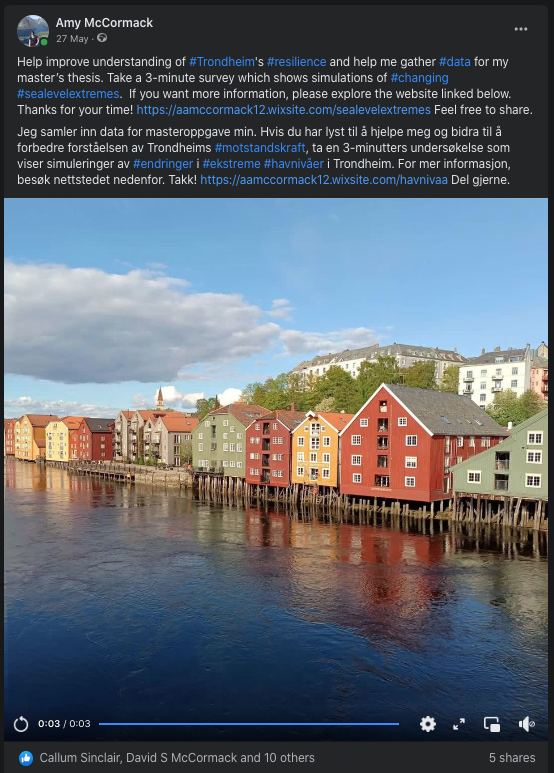
\includegraphics[width=0.7\textwidth]{fig_appendix/so_me.png}
    \caption{Social Media Post Used to Reach Subjects}{A short video playing a loop of the simulated water level extremes in Nidelva was utilised to optimise algorithms which prioritise video.}
    \label{fig:my_label}
\end{figure}


\begin{figure}[H]
    \centering
    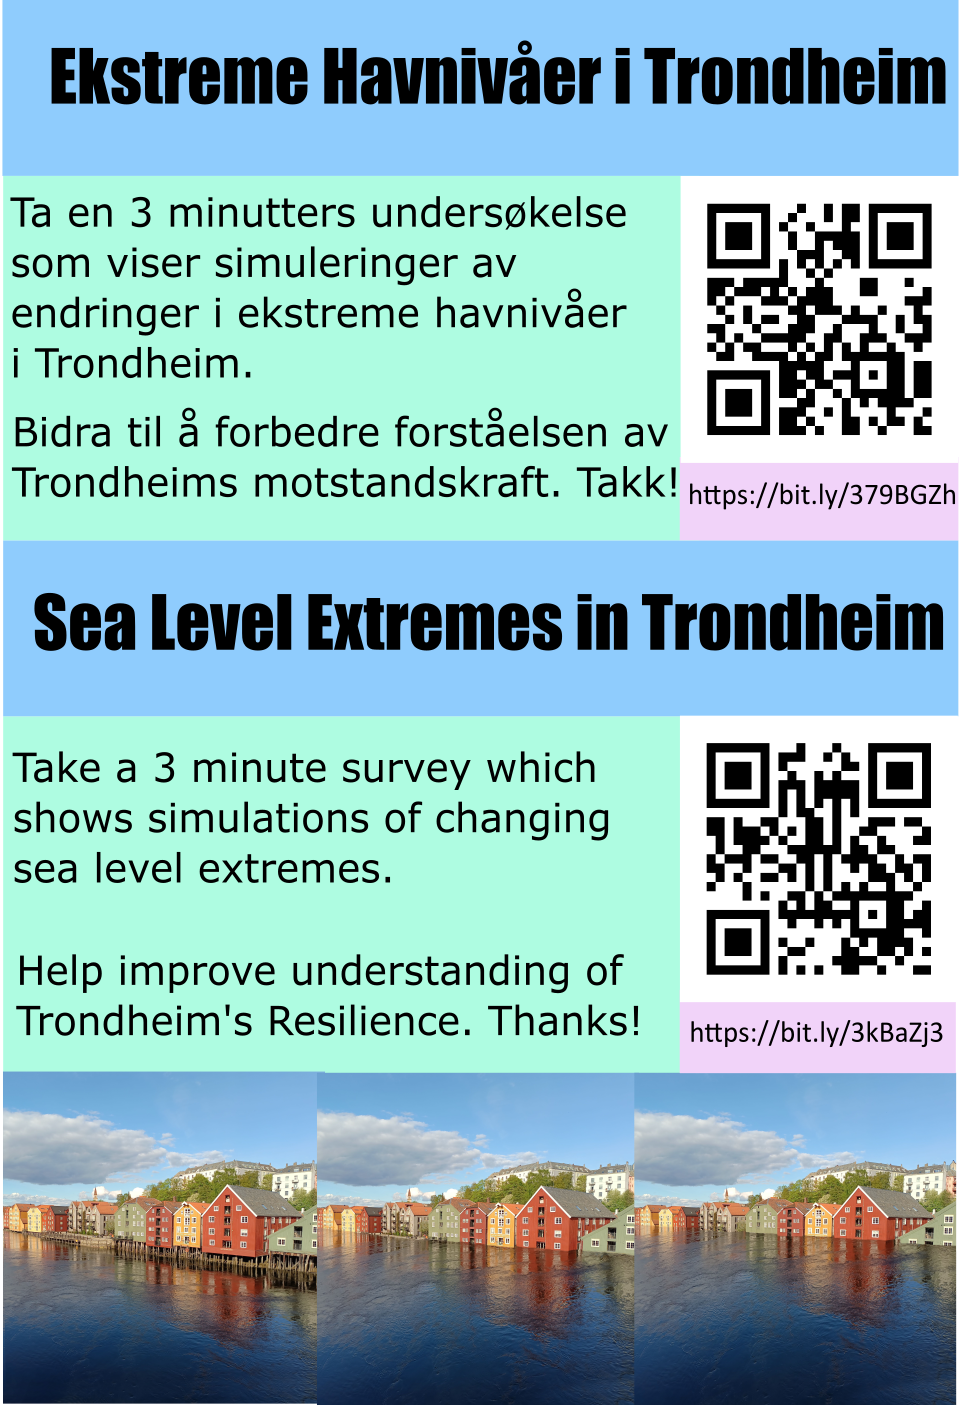
\includegraphics[width=0.9\textwidth]{fig_appendix/poster-larger.png}
    \caption{This is the poster used to reach subjects}
    \label{fig:poster}
\end{figure}

\subsection{Example Emails}
\textbf{In English}

Hi [NAME],
\paragraph{}
I am researching extreme sea level changes in Trondheim, and the population's knowledge about it. If you want to help me and possibly help improve the understanding of Trondheim's resilience, feel free to take a 3-minute survey that shows simulations of changes in extreme sea levels in Trondheim, and share it with your colleagues. 
\paragraph{}
For more information and the survey, visit the website below. Thanks! \url{https://aamccormack12.wixsite.com/havnivaa} (Norwegian) \url{https://aamccormack12.wixsite.com/sealevelextremes} (English)
\paragraph{}
If you have any questions about the research or other things, feel free to get in touch.
\paragraph{}
With best regards
\newline
Amy Anne McCormack
\paragraph{}
amymc@stud.ntnu.no
\paragraph{}

\textbf{In Norwegian}

Hei [NAVN],
\paragraph{}
Jeg forsker på ekstrem havnivåendringer i Trondheim, og befolkningens vitenskap om det.  Jeg er spesielt interessert i svar fra folk som jobber innom marine roller.
\paragraph{}
Hvis du har lyst til å hjelpe meg og bidra til å forbedre forståelsen av Trondheims motstandskraft, kan du gjerne ta en 3-minutters undersøkelse som viser simuleringer av endringer i ekstreme havnivåer i Trondheim, og dele det med dine kolleger.
\paragraph{}
For mer informasjon og undersøkelsen, besøk nettstedet nedenfor. Takk! \url{https://aamccormack12.wixsite.com/havnivaa}
\paragraph{}
Hvis du har noen spørsmål om forskningen eller masteroppgaven minn, ta gjerne kontakt.
\paragraph{}
 

Med vennlig hilsen 
\newline
Amy Anne McCormack
\paragraph{}
amymc@stud.ntnu.no



% Include more appendices as required.
%%=========================================
\bibliographystyle{apa}
\addcontentsline{toc}{chapter}{\bibname}
\bibliography{refs}  
%%=========================================

\end{document}
